% !TeX root = ../main.tex

\chapter{结果与分析}

\section{系统成果}

当前决赛版本在初赛工作的基础上，实现了一个面向比赛提交和现场演示的完整透明泡泡渲染与交互系统。主要成果包括：

\subsection{渲染与光学}

\begin{itemize}
  \item 通过多阶段FBO近似双界面折射，背景参照物和天空盒能在泡泡中产生明显扭曲。
  \item 三种薄膜虹彩模式已在Native层实现：Kim2012实时三波长公式计算、Spectral LUT预计算纹理查表、Belcour Airy多波长Airy反射近似。界面开放Kim与Airy两种展示模式，便于说明实时公式与多波长近似之间的差异。
  \item 动态膜厚让虹彩随时间缓慢流动，不依赖静态纹理。程序化膜厚由多层Simplex噪声、排液趋势项和触摸扰动共同生成，使用世界法线方向（而非UV坐标）作为噪声输入，避免球体UV接缝处的明显断裂。
\end{itemize}

\subsection{多泡泡交互}

\begin{itemize}
  \item 基于空间哈希和接触图的多泡泡仿真框架：支持运行时动态创建与删除泡泡，泡泡数量可变（默认上限8，硬上限16）。
  \item 接触激活函数实现从接近、预接触、成膜到结果锁定的平滑过渡，避免单帧状态切换。
  \item 接触圆弹簧-阻尼动力学与多接触位置约束迭代（每帧6次），支持一个泡泡同时参与多条接触关系。
  \item 每泡26个持久表面控制点，弹簧-阻尼更新，支持多接触变形聚合、接触帽压缩和接触环鼓包。
  \item Young-Laplace弯曲共享膜：等尺寸泡泡间为平面膜，不等尺寸时膜向大泡（低压）一侧弯曲，使用解析球冠表示且边界始终与原接触平面对齐。
  \item 三种接触结果：分离（粘结合约释放后柔性分离）、稳定8字双泡（独立腔体，共享膜保留）、融合（小泡被大泡吸收，体积守恒）。
  \item 泡泡身份使用稳定BubbleId，支持运行时增删而不导致模型错位。
\end{itemize}

\subsection{动力学与交互}

\begin{itemize}
  \item 方向性风场：可调节强度与方向，小泡泡响应更强，关闭后速度阻尼平滑衰减。
  \item 每泡DBSTT涡流片仿真：泡泡破裂时激活，膜回缩由涡流片物理模型驱动而非预设动画。
  \item 两套预置演示场景：综合开场场景（Scene按钮）和双泡专项循环演示（Demo按钮），覆盖稳定双泡、融合、分离三种典型交互。
  \item 完整HarmonyOS端触控与界面交互，支持动态生成、删除、参数调节和场景切换。
\end{itemize}

\subsection{工程完整性}

\begin{itemize}
  \item HarmonyOS工程（ArkTS页面 + NAPI接口 + Native渲染层）和Windows桌面工程（GLFW + OpenGL）已形成完整的双平台开发与提交链路。
  \item 可执行HAP程序已整理入提交目录。
\end{itemize}

\subsection{移动端交互界面}

\begin{center}
  \centering
  \begin{minipage}[t]{0.46\linewidth}
    \centering
    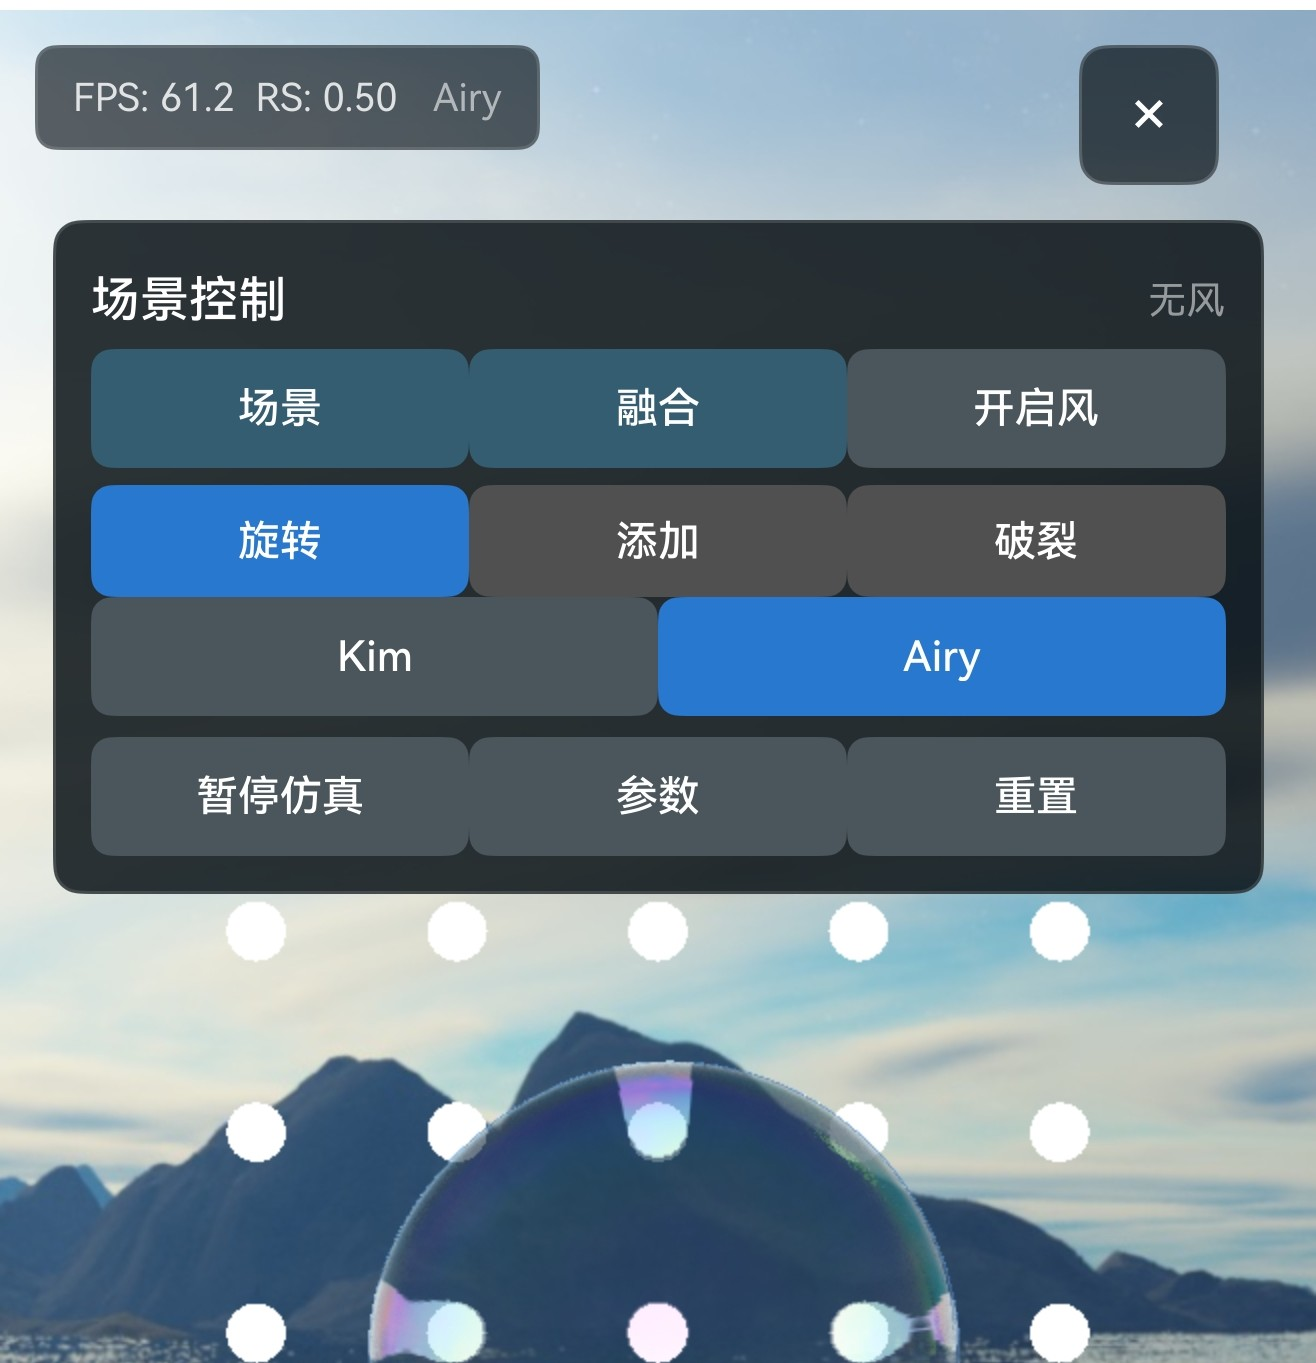
\includegraphics[width=\linewidth,height=0.28\textheight,keepaspectratio]{figures/UI界面.jpg}\\[0.3em]
    \small 场景控制菜单
  \end{minipage}
  \hfill
  \begin{minipage}[t]{0.46\linewidth}
    \centering
    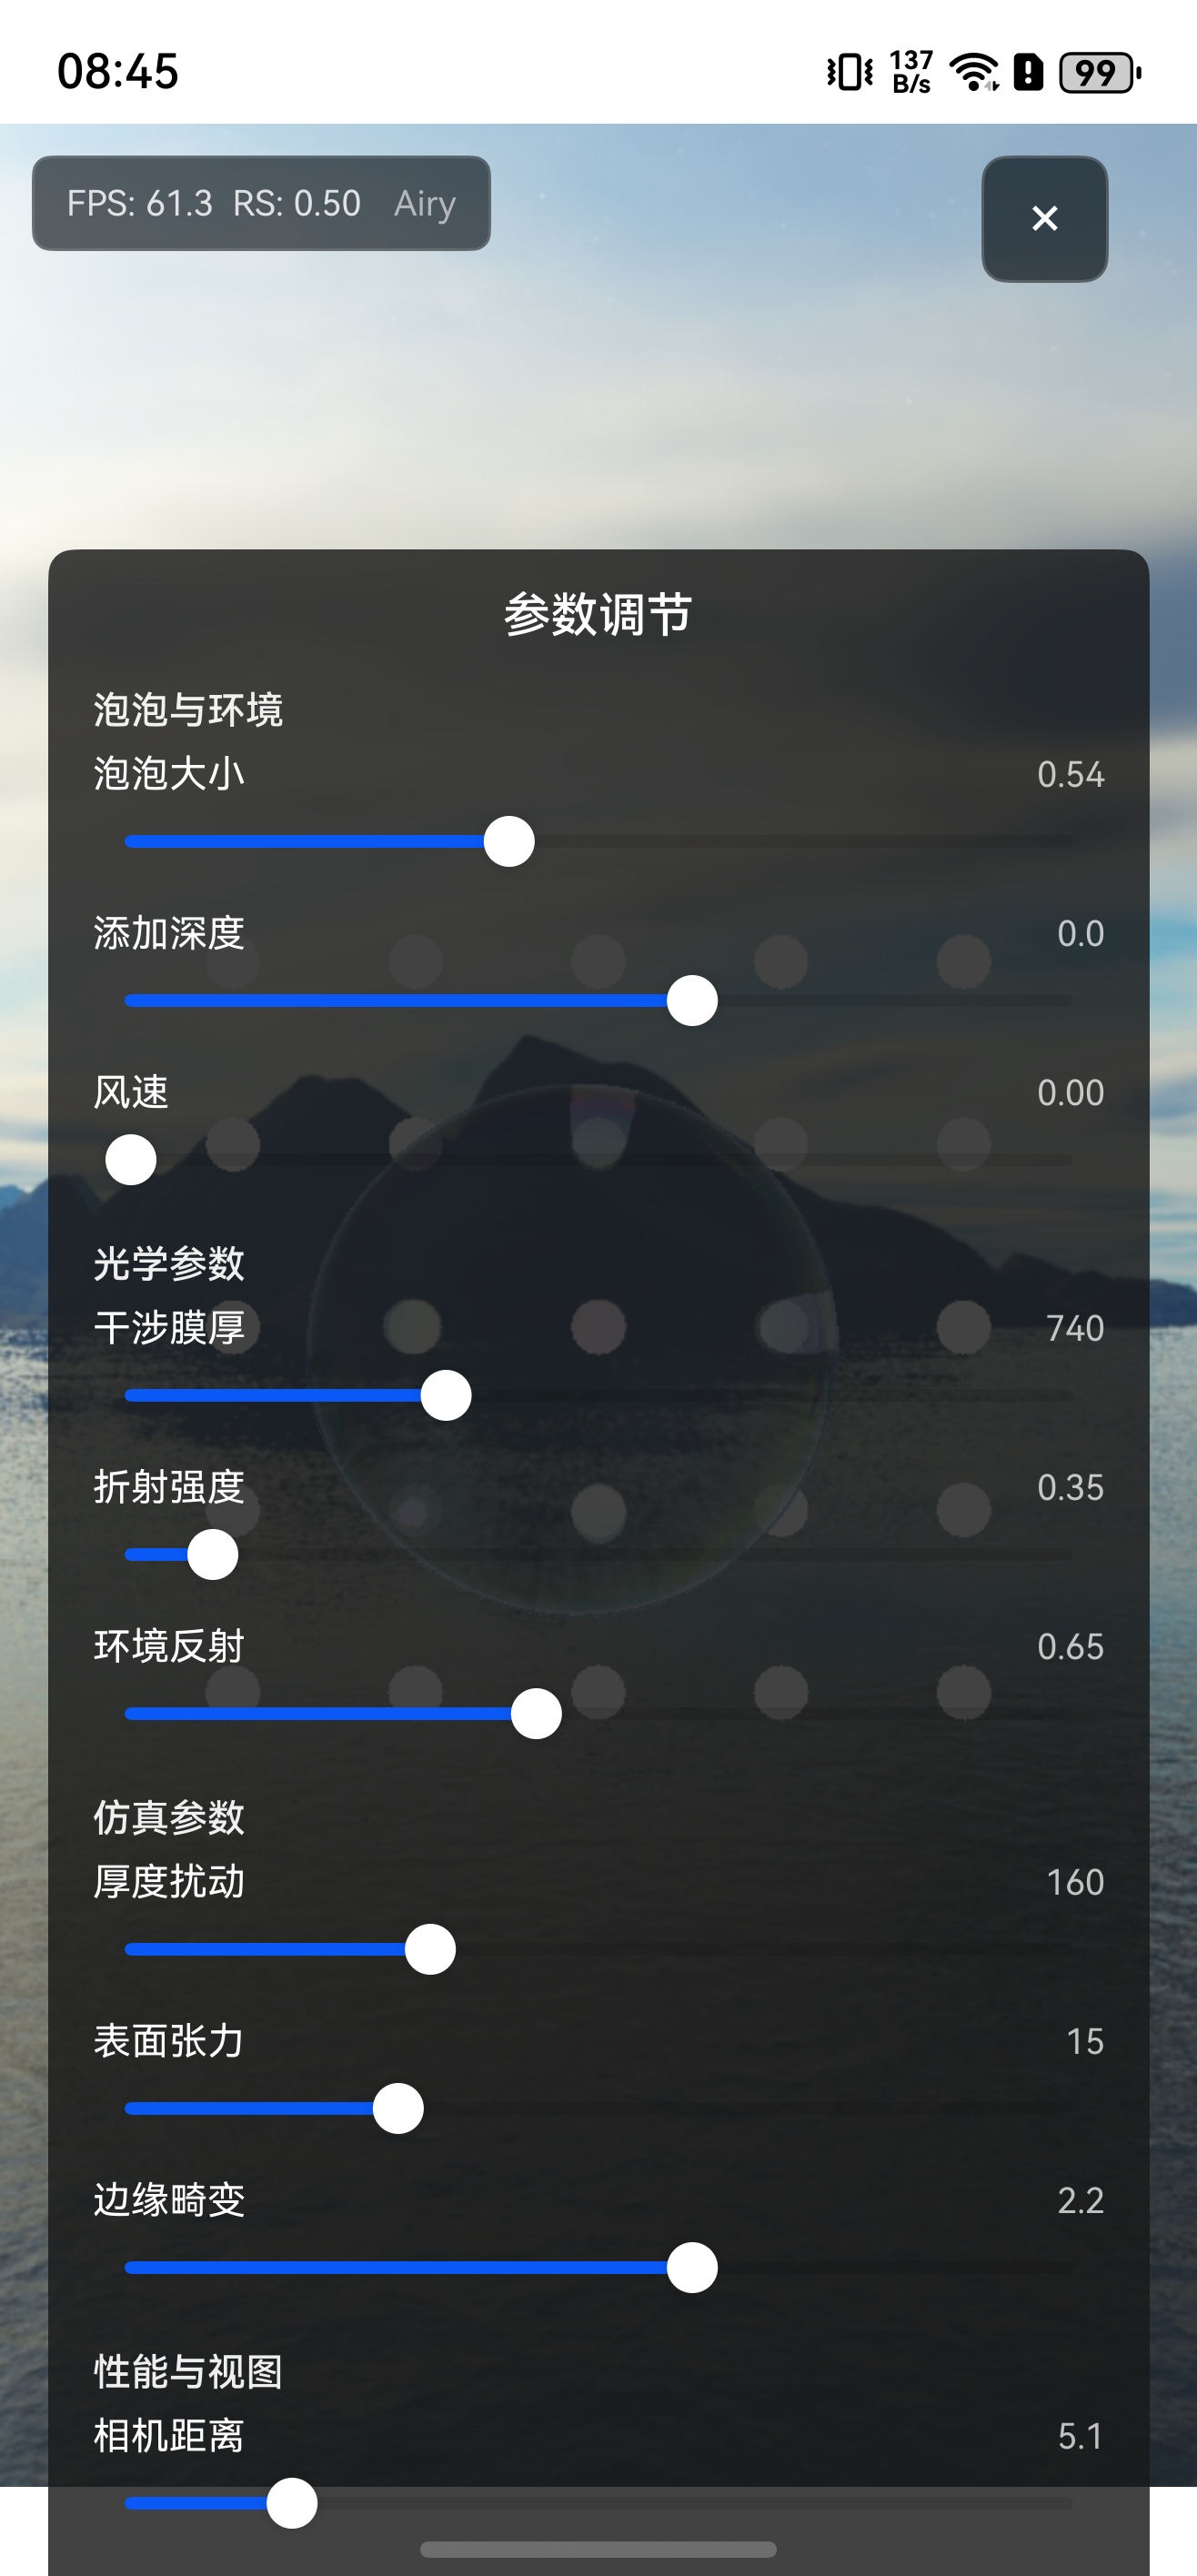
\includegraphics[width=\linewidth,height=0.28\textheight,keepaspectratio]{figures/参数调节.jpg}\\[0.3em]
    \small 参数调节面板
  \end{minipage}
  \captionof{figure}{HarmonyOS端的场景控制与参数调节界面}
  \label{fig:mobile_ui}
\end{center}

\section{效果展示}

\subsection{多泡泡接触场景}

\begin{figure}[H]
  \centering
  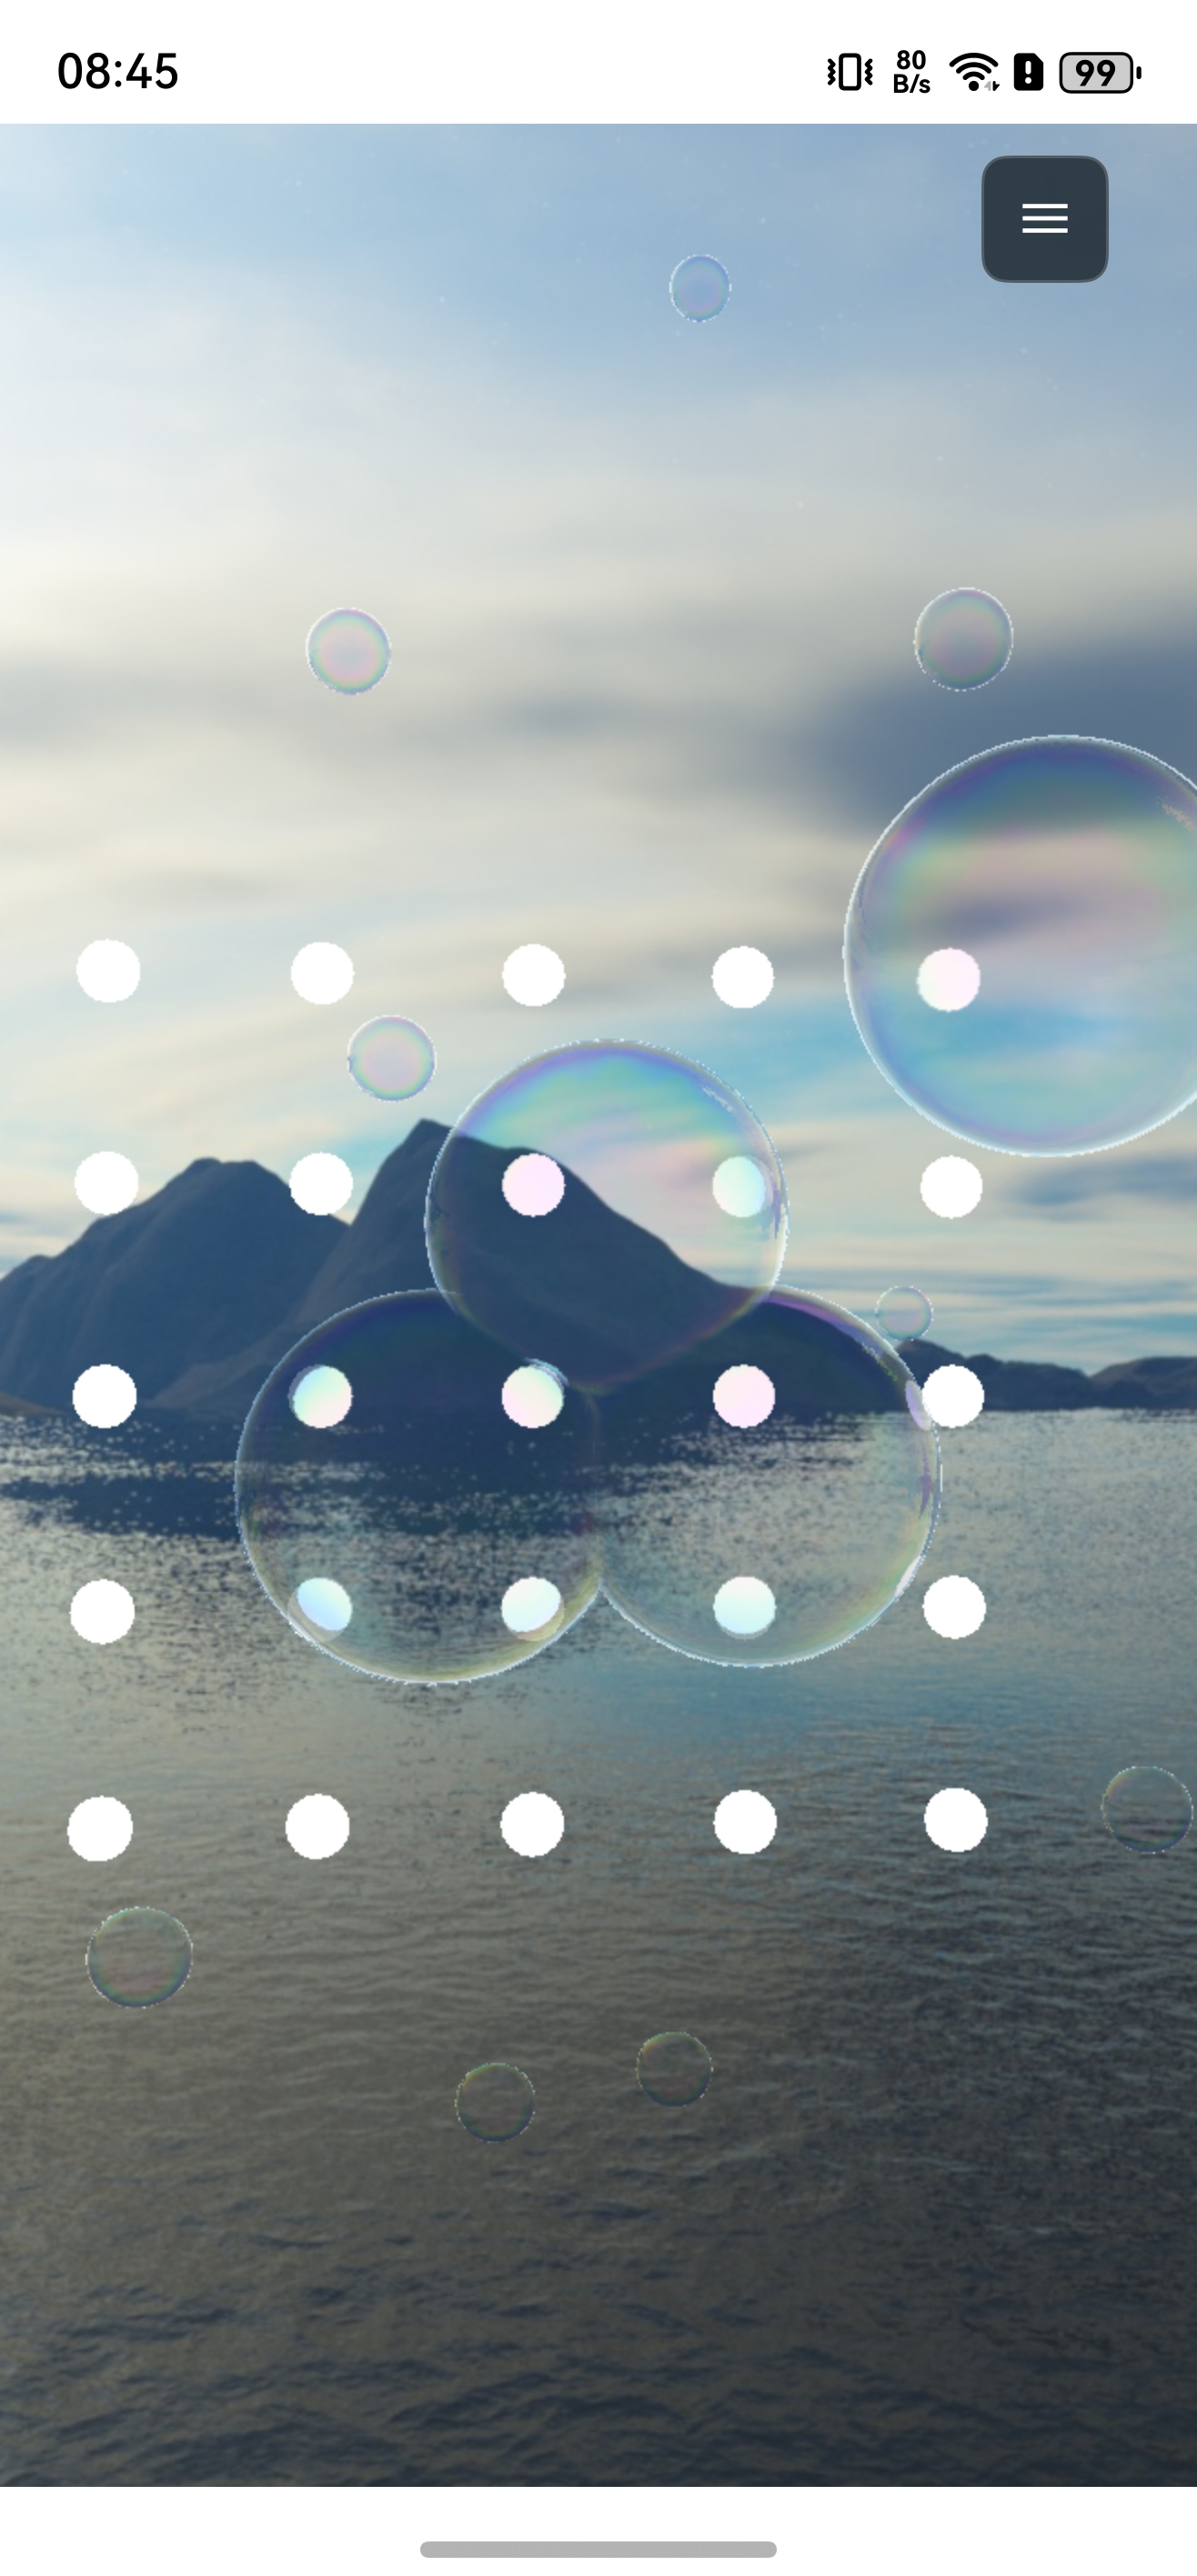
\includegraphics[width=0.72\linewidth,height=0.23\textheight,keepaspectratio]{figures/6.1.jpg}
  \caption{多泡泡接触场景：三个真实模拟泡泡形成接触网络，右侧为融合结果，左侧为独立泡泡}
\end{figure}

\subsection{三种接触结果对比}

\begin{figure}[H]
  \centering
  \begin{minipage}[t]{0.30\linewidth}
    \centering
    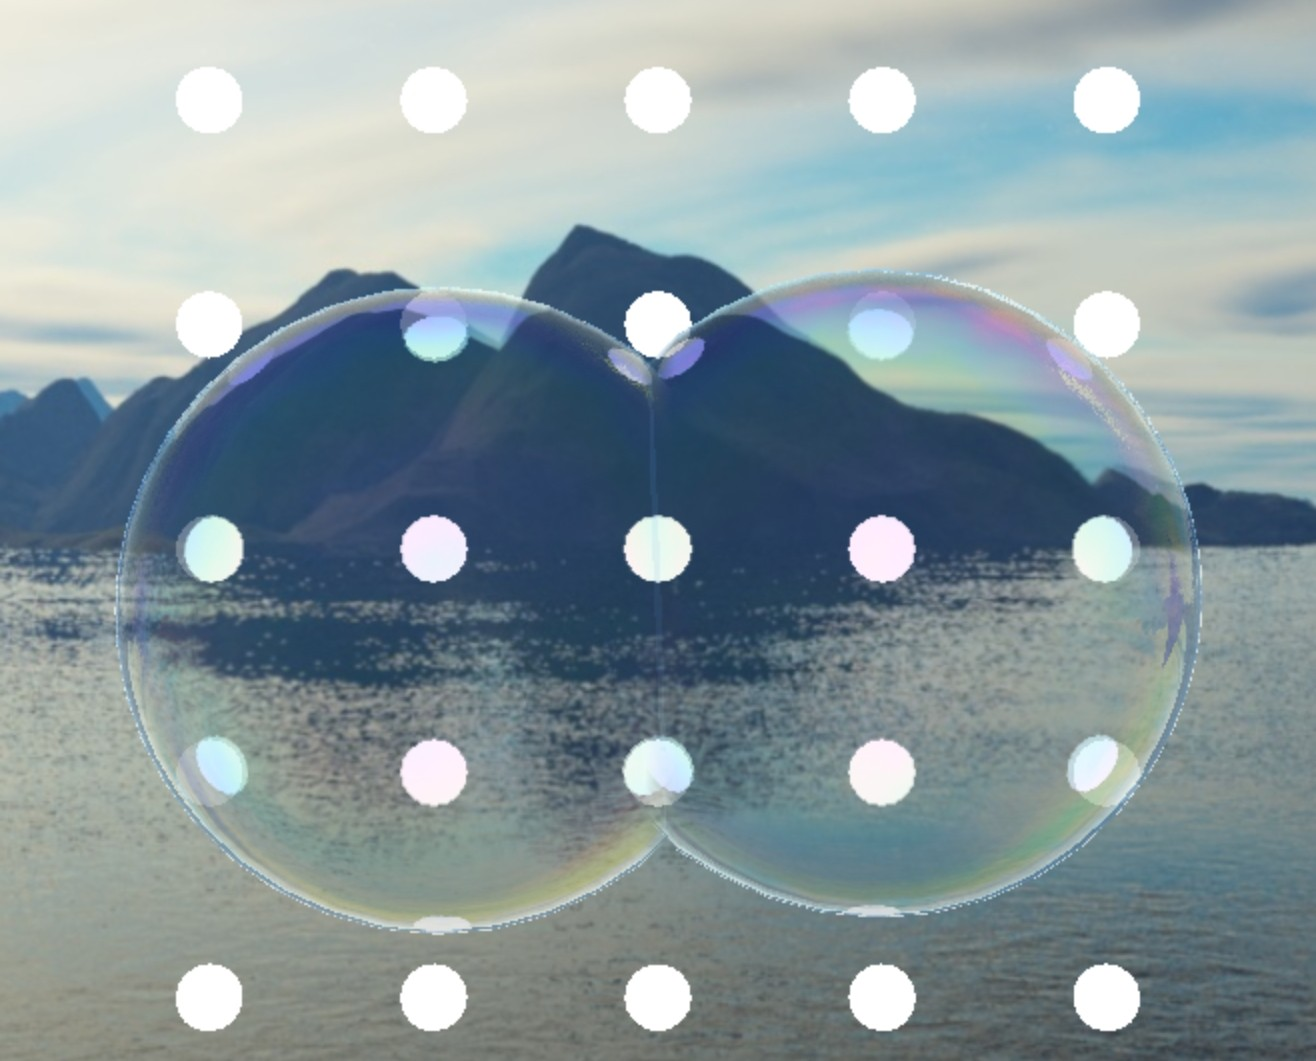
\includegraphics[width=\linewidth,height=0.22\textheight,keepaspectratio]{figures/6.3a.jpg}\\[0.3em]
    \small (a) 分离
  \end{minipage}
  \hfill
  \begin{minipage}[t]{0.30\linewidth}
    \centering
    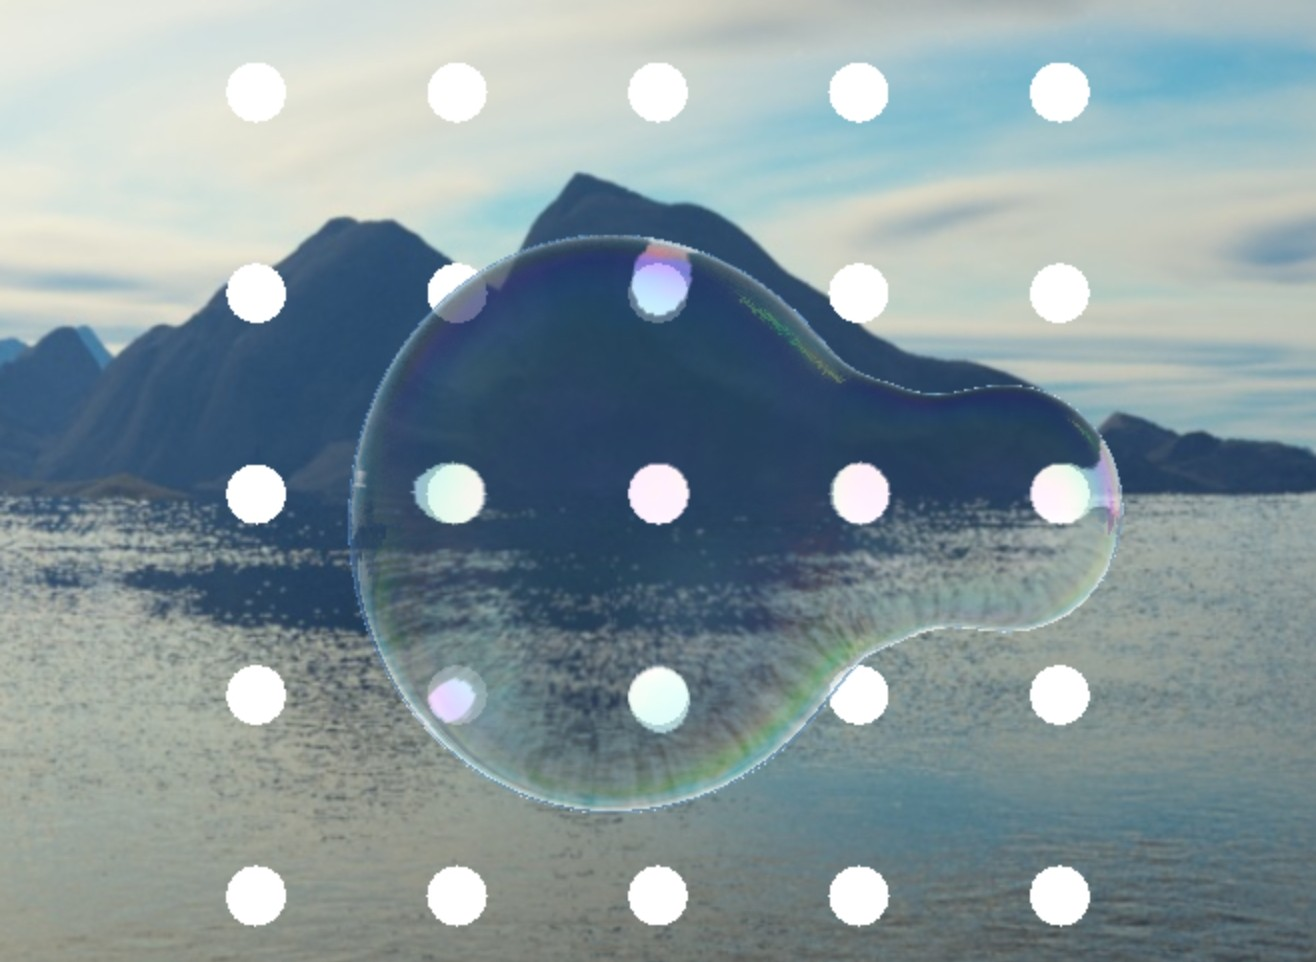
\includegraphics[width=\linewidth,height=0.22\textheight,keepaspectratio]{figures/6.3b.jpg}\\[0.3em]
    \small (b) 稳定双泡
  \end{minipage}
  \hfill
  \begin{minipage}[t]{0.30\linewidth}
    \centering
    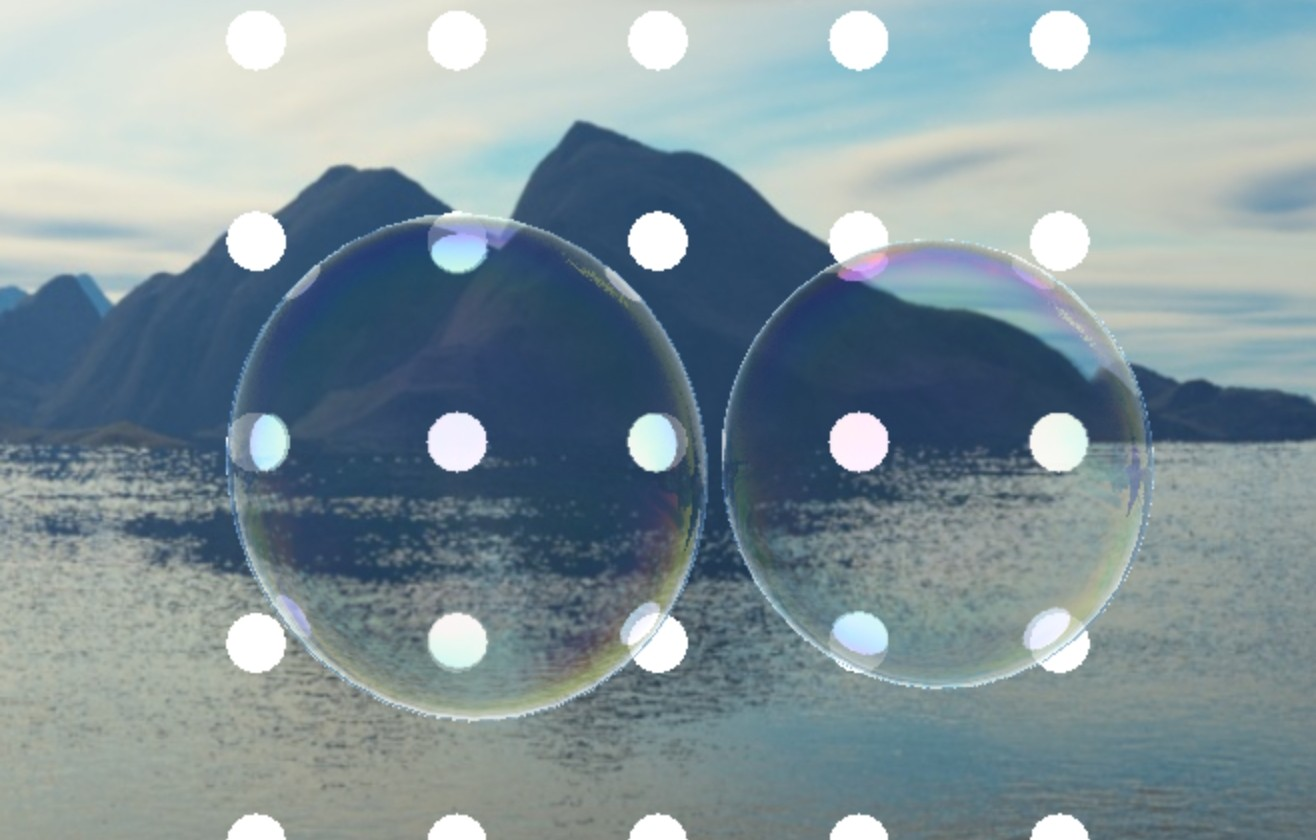
\includegraphics[width=\linewidth,height=0.22\textheight,keepaspectratio]{figures/6.3c.jpg}\\[0.3em]
    \small (c) 融合
  \end{minipage}
  \caption{三种接触结果对比}
  \label{fig:three_outcomes}
\end{figure}

\section{性能分析}

系统在Windows桌面端（Release构建）和HarmonyOS设备上均能稳定运行。由于桌面端为开发调试环境，此处以HarmonyOS端性能为主要参考。

\begin{table}[H]
  \centering
  \caption{性能参考数据}
  \begin{tabular}{p{0.35\linewidth}p{0.25\linewidth}p{0.25\linewidth}}
    \toprule
    场景 & 泡泡数 & 帧率（FPS） \\
    \midrule
    单泡泡（DBSTT仿真） & 1 & 约60 \\
    综合开场场景 & 8+ & 约30 \\
    双泡泡接触交互演示 & 2 & 约50 \\
    \bottomrule
  \end{tabular}
\end{table}

以上性能数据在华为 Mate 70 Pro 真机上测得。主要性能开销来源：
\begin{itemize}
  \item 多阶段FBO合成（每帧至少5个pass）；
  \item 接触图位置约束迭代（$O(K \cdot I)$，其中$K$为接触边数，$I=6$为迭代次数）；
  \item 每泡表面控制点更新（$O(N \cdot C)$，$N$为泡泡数，$C=26$为控制点数）；
  \item DBSTT涡流片仿真的Biot-Savart速度求解（$O(V \cdot T)$，$V$为顶点数，$T$为三角形数）。
\end{itemize}

\section{局限与展望}

当前系统存在以下明确局限：

\begin{itemize}
  \item \textbf{屏幕空间折射的固有局限}：不能表现屏幕外物体，也不能严格模拟多泡泡之间的相互折射。
  \item \textbf{Plateau border缺失}：多接触相交处尚未形成符合表面张力平衡的120度交汇结构，共享膜在中央可能互相穿过或留下缝隙。
  \item \textbf{膜厚为标量}：每个接触对只有一个膜厚值，无法表达重力排液、局部黑膜和接触区域材料交换。
  \item \textbf{透明排序}：泡泡数量增加后，固定距离排序+alpha混合可能出现顺序错误和黑带。
  \item \textbf{Shader接触平面数量限制}：球壳shader最多接收四个接触平面，限制了一个泡泡的最大邻居数。
  \item \textbf{融合概率模型}：当前基于尺寸比、接触时间等的经验概率模型，不是完整膜排液或流体求解器。
  \item \textbf{DBSTT简化}：仿真仅用于单闭合泡泡，不支持原论文中的泡沫拓扑变化和Plateau边界。
  \item \textbf{Belcour Airy简化}：是实时shader中的项目级简化，不包含完整微表面模型和解析光谱预积分。
\end{itemize}

后续迭代的优先方向：
\begin{enumerate}
  \item 实现多泡泡之间的相互折射和反射，提升多泡泡场景的光学真实感。
  \item 建立显式的ContactPatch边界环和PlateauBorder，使多接触交汇处符合物理规律。
  \item 实现低分辨率二维膜厚场，支持排液、颜色流和接触区材料交换。
  \item 采用weighted blended OIT或两层depth peeling改善透明排序。
  \item 将接触数据从uniform数组扩展至texture buffer或SSBO，支持任意数量的邻居。
  \item 实现严格的封闭三角网格体积积分与投影，支持更深挤压和动态拓扑变化。
\end{enumerate}

\section{总结}

本项目从透明肥皂泡的主要视觉现象出发，实现了一个面向赛题二决赛提交的HarmonyOS渲染系统。渲染方面，项目通过多阶段FBO合成近似双界面折射，实现了Kim2012、Spectral LUT和Belcour Airy三种薄膜虹彩模式。动力学方面，项目构建了以接触图为核心的多泡泡交互框架：引入空间哈希加速、连续接触激活、接触圆弹簧-阻尼动力学、持久表面控制点变形、Young-Laplace弯曲共享膜，以及分离/稳定双泡/融合三种接触结果。辅助系统包括方向性风场、每泡DBSTT涡流片仿真、动态泡泡增删和两套预置演示场景。

系统在HarmonyOS和Windows双平台均形成完整的开发与演示链路。决赛版本将初赛的单泡泡展示系统扩展为真正意义上的多泡泡交互仿真平台，使最终结果更符合比赛对"效果、交互、完整性"的要求。
